\documentclass[11pt,letterpaper]{article}

% --- packages ---------------------------------------------------------------
\usepackage[margin=1in]{geometry}
\usepackage{amsmath,amssymb,amsthm}
\usepackage{graphicx}
\usepackage{booktabs}
\usepackage{multirow}
\usepackage{array}
\usepackage{xcolor}
\usepackage{caption}
\usepackage{subcaption}
\usepackage[hidelinks,colorlinks=true,linkcolor=blue!50!black,citecolor=blue!50!black,urlcolor=blue!50!black]{hyperref}
\usepackage{natbib}
\usepackage{authblk}
\usepackage{enumitem}
\usepackage{siunitx}
\usepackage{microtype}

\graphicspath{{../figures/}{./figures/}}

% --- macros -----------------------------------------------------------------
\newcommand{\Vart}{\operatorname{Var}}
\newcommand{\CVaR}{\operatorname{CVaR}}
\newcommand{\E}{\mathbb{E}}
\newcommand{\AC}{Almgren--Chriss}
\newcommand{\HJB}{HJB}

% --- title ------------------------------------------------------------------
\title{Optimal Execution under Stochastic Volatility on \\
       Binance BTCUSDT: Calibration, HJB Solver, and Regime Awareness}

\author[1]{Eva-Qi}
\author[1]{bp}
\author[1]{Yuhao}

\affil[1]{MF796 Computational Methods of Mathematical Finance, Boston University}

\date{\today}

\begin{document}
\maketitle

% ============================================================================
\begin{abstract}
\noindent
We implement the \citet{almgren2001optimal} optimal-execution framework on real Binance BTCUSDT data, calibrate market-impact parameters from \(98\) days of \(\sim 130\)M aggregated trades, and extend the model along three axes: (B) a fully implicit \HJB{} PDE solver with Howard's policy iteration for nonlinear temporary impact, (D) a Heston Q-measure stochastic-volatility extension calibrated by Carr--Madan FFT \citep{carr1999option} against the Deribit BTC option implied-volatility surface, and (E) a two-state Hidden Markov regime-aware execution scheduler. A code-council audit caught a silent bid-ask-bounce bias that produced economically nonsensical \(\gamma = -0.0113\) at the tick level; a 1-min~\(\to\)~5-min~\(\to\)~tick~\(\to\)~literature-fallback cascade restores \(\gamma=+1.48\) (\(R^2=0.18\)), \(\eta=1.58\!\times\!10^{-4}\), \(\alpha=0.441\), all in literature ranges. An independent order-book-depth integral yields \(\eta\approx1.58\!\times\!10^{-4}\), confirming the cascade. The Heston Q-measure calibration is stable across 12 monthly snapshots (\(\operatorname{std}(\kappa)=0.01\), \(\operatorname{std}(\rho)=0.001\); IV-surface RMSE \(=0.0086\)) and outperforms the 3/2 model by 33.9\% RMSE on the same chain. Walk-forward six-split out-of-sample validation at \(X_0=1000\) BTC shows AC beats TWAP by \(15.1\%\)--\(36.9\%\) MC savings across all six splits (\(p<0.0001\)). On a CRN-coupled paired Monte Carlo test of 10\,000 paths, the Heston-Q-aware schedule reduces \(\CVaR_{95}\) by \(14.59\%\) versus constant-vol (\(p<0.0001\)). The regime-aware extension underwent five iterative refinements (V1--V5); we document each version's bias layer and report that V4's positive finding (\(\CVaR_{95}\) \(-14.0\%\), \(p<0.0001\)) was \emph{invalidated} by V5's true per-regime OLS calibration, which sign-reversed the result. The regime-aware claim remains unresolved on the 98-day window; a 280-day extension (V6) is in flight. We close with five audit-mechanism lessons --- numerical convention drift, two-solver cross-check, dead-code accumulation, calibration identification, and proxy-vs-direct-data --- that were essential for surfacing every result in this paper.

\medskip
\noindent\textbf{Keywords:} optimal execution; Almgren--Chriss; Heston stochastic volatility; Hidden Markov Model; Hamilton--Jacobi--Bellman equation; cryptocurrency market microstructure; market impact calibration; tail risk
\end{abstract}

% ============================================================================
\section{Introduction}
\label{sec:intro}

The optimal-execution problem --- liquidating \(X_0\) units of an asset over a finite horizon \([0,T]\) while balancing market-impact cost against price-risk variance --- has a textbook solution under the \citet{almgren2001optimal} framework when impact is linear and volatility is constant. Real markets violate both assumptions. Cryptocurrency markets in particular feature regime-dependent volatility, leverage effects, and a power-law impact exponent \(\alpha<1\) that breaks the separable closed-form ansatz \(V(t,x)=a(t)x^2\) underlying the canonical solution. This paper asks: \emph{what changes when we replace the constant-volatility assumption with calibrated Heston dynamics, and what changes when we replace the static execution schedule with a regime-aware scheduler driven by a Hidden Markov Model?}

We make three contributions. \textbf{First}, we calibrate \AC{} permanent-impact \(\gamma\), temporary-impact coefficient \(\eta\), and impact exponent \(\alpha\) from real Binance BTCUSDT trade and order-book data, after diagnosing and correcting a bid-ask-bounce bias that produced negative permanent impact at the tick level. The fix is a multi-tier aggregation cascade in \texttt{calibration/impact\_estimator.py}, validated by an independent order-book-depth estimator. \textbf{Second}, we develop a fully implicit \HJB{} PDE solver in \texttt{pde/hjb\_solver.py} that uses closed-form Riccati for \(\alpha=1\) and Howard's policy iteration with Crank--Nicolson discretization for \(\alpha\neq1\); we cross-check the solver against an SLSQP-based discrete-trade-vector optimizer. \textbf{Third}, we extend the model to stochastic volatility (Heston Q-measure, calibrated against Deribit option implied-volatility surfaces by Carr--Madan FFT) and to regime awareness (a two-state Gaussian HMM on five-minute log-returns). For each extension we run paired Monte Carlo tests with common-random-numbers coupling at \(X_0=1000\) BTC and report effect sizes alongside \(p\)-values.

\textbf{Methodologically}, we found that an audit-first development style --- explicit numerical-convention checks, two-solver cross-verification, dead-code retirement, and calibration-identification audits --- caught four classes of bug that were invisible to standard \texttt{pytest} unit testing. We close the paper with a brief synthesis of those audit mechanisms because each was essential to producing the headline results. The remainder of this paper is organized as follows. Section~\ref{sec:background} reviews the \AC{} framework and the Heston/HMM extensions. Section~\ref{sec:data} describes the dataset and calibration procedure. Sections~\ref{sec:hjb}--\ref{sec:regime} present the HJB solver, Heston extension, and regime-aware extension respectively. Section~\ref{sec:audit} synthesizes the methodological learnings. Section~\ref{sec:limitations} discusses limitations and future work; Section~\ref{sec:conclusion} concludes.

% ============================================================================
\section{Background and Related Work}
\label{sec:background}

\subsection{The Almgren--Chriss optimal-execution problem}

\citet{almgren2001optimal} formulate optimal execution as a mean-variance trade-off. Given an inventory \(X(t)\) to liquidate over \([0,T]\) with trading rate \(v(t) = -\dot{X}(t)\), the asset price evolves as
\begin{equation}
\label{eq:price}
dS_t = -\gamma\, v(t)\, dt + \sigma\, dW_t,
\end{equation}
where \(\gamma\) is the \emph{permanent-impact} coefficient (Kyle's \(\lambda\) generalized) and \(\sigma\) is the (annualized) instantaneous volatility. The execution cost is
\begin{equation}
\label{eq:cost}
C = \int_0^T \big[\, \gamma\, v(t)\, X(t) + \eta\, |v(t)|^{\alpha}\, \big]\, dt,
\end{equation}
where \(\eta\, |v|^{\alpha}\) is the \emph{temporary-impact} cost; \(\alpha=1\) recovers the linear original of \citet{almgren2001optimal}, and \(0<\alpha<1\) corresponds to the empirically-observed power-law impact \citep{almgren2003optimal,gatheral2010no}. The execution objective is
\begin{equation}
\label{eq:obj}
\min_{v(\cdot)}\; \E[C] + \lambda\, \Vart[C],
\end{equation}
where \(\lambda\geq 0\) is the trader's risk aversion. For \(\alpha=1\) the solution is the classical \(\sinh(\kappa t)\) trajectory with \(\kappa = \sqrt{\lambda\sigma^2/\eta}\). For \(\alpha\neq 1\) the separable ansatz fails and one must solve the HJB equation directly \citep{schied2010optimal}.

\subsection{Stochastic volatility (Heston)}

The \citet{heston1993closed} model couples spot and instantaneous variance:
\begin{align}
\label{eq:heston}
dS_t &= \mu S_t\, dt + \sqrt{v_t}\, S_t\, dW_t^{(1)},\\
dv_t &= \kappa(\theta - v_t)\, dt + \xi\sqrt{v_t}\, dW_t^{(2)},\\
\E[dW^{(1)}_t\, dW^{(2)}_t] &= \rho\, dt.
\end{align}
With \(\rho<0\) the model captures the leverage effect (vol up when price down). The standard pricing tool is the Carr--Madan FFT \citep{carr1999option}, which inverts the characteristic function to produce a fast option-price grid for calibration.

\subsection{Hidden Markov regime detection}

\citet{hamilton1989new} introduced the regime-switching framework where observed returns \(r_t\) are emissions from a latent Markov chain \(z_t \in \{1,\ldots,K\}\). For \(K=2\) (risk-on/risk-off), each state has its own mean and volatility; the \citet{baum1970maximization} algorithm fits parameters and \citet{viterbi1967error} decodes the most likely state sequence. We use the \texttt{hmmlearn} GaussianHMM implementation throughout.

% ============================================================================
\section{Data and Calibration}
\label{sec:data}

\subsection{Data sources}

We use three primary data sources, described in Table~\ref{tab:data}. The Binance aggTrades stream covers 98 calendar days (2026-01-01 through 2026-04-08, approximately 130 million trade prints) and provides the basis for trade-level calibration of \(\gamma\), \(\eta\), \(\alpha\), and the realized-volatility \(\sigma\). The Tardis monthly Deribit option chain snapshots span 2025-05 through 2026-04 and are used for the 12-month Heston calibration time series. The Deribit live chain snapshots (2026-04-20 and 2026-04-21) anchor the canonical Heston Q-measure calibration via Carr--Madan FFT.

\begin{table}[!htb]
\centering
\caption{Data sources and their canonical roles. CRN = common-random-numbers coupling; bookDepth coverage is 28 days, archived locally for the robustness paragraph (Section~\ref{sec:bookdepth}) but not part of the canonical pipeline.}
\label{tab:data}
\small
\begin{tabular}{l l l l}
\toprule
\textbf{Source} & \textbf{Coverage} & \textbf{Role} & \textbf{Status} \\
\midrule
Binance aggTrades & 98 days, \(\sim130\)M trades & \(\gamma,\eta,\alpha,\sigma\) calibration & active (canonical) \\
Tardis Deribit options (BTC) & 12 monthly snapshots & 12-month Heston \(\kappa/\rho/\theta/\xi\) stability & active (cross-check) \\
Deribit live option chain & 2 daily snapshots & Carr--Madan FFT calibration anchor & active (canonical) \\
Coinbase 5-min klines & 98 days & Cross-exchange spot proxy + realized \(\rho\) & auxiliary \\
Binance 1d klines & 98 days & Daily realized volatility & active \\
Binance bookDepth (28d) & 28 days & Direct \(\eta\) cross-check & robustness only \\
FRED + CoinMetrics & 98 days & HMM exogenous-feature ablations (rejected) & null result \\
\bottomrule
\end{tabular}
\end{table}

\subsection{Almgren--Chriss parameter calibration}
\label{sec:calibration}

The original tick-level Kyle's-\(\lambda\) regression \(\Delta S_t = -\gamma\, v_t + \varepsilon_t\) returned \(\hat\gamma = -0.0113\), an economically impossible \emph{negative} permanent impact. Diagnosis: at the tick level, \(\Delta S_t\) is dominated by bid-ask-bounce noise --- a buy-print at the ask is followed by a sell-print at the bid even with no information arrival, inducing a spurious negative correlation between trade direction and next-print return. The temporary-impact estimator \(\hat\eta\, |v|^{\hat\alpha}\) suffered the same bias, returning \(\hat\alpha\approx 0.04\), well below the literature range of \([0.3, 1.5]\) \citep{almgren2003optimal,gatheral2010no}.

The fix is a multi-tier aggregation cascade in \texttt{calibration/impact\_estimator.py}: try 1-min bars first, accept if \(R^2>0.05\) and the parameter is in literature range; otherwise fall back to 5-min, then to tick, then to literature constants \(\gamma=10^{-4}\), \(\eta=10^{-3}\), \(\alpha=0.6\). The first tier hits and produces the production estimates in Table~\ref{tab:calib}. The 1-min aggregation averages out bid-ask-bounce while preserving the directional information that drives genuine impact.

\begin{table}[!htb]
\centering
\caption{Calibration cascade results on Binance BTCUSDT, 98 days (2026-01-01 to 2026-04-08). The tick-level row is included to show what the raw estimator returns before aggregation; only the 1-min row is used in production. The bookDepth row is an independent estimator on 28 days of order-book-depth data; agreement at \(\eta\approx 1.58\!\times\!10^{-4}\) is the robustness check (Section~\ref{sec:bookdepth}).}
\label{tab:calib}
\small
\begin{tabular}{l c c c c l}
\toprule
\textbf{Method} & \(\bm\gamma\) & \(\bm\eta\) & \(\bm\alpha\) & \(\bm{R^2}\) & \textbf{Verdict} \\
\midrule
Tick-level (original) & \(-0.0113\) & \(1.7\!\times\!10^{-5}\) & \(0.04\) & \(0.001\) & bid-ask bounce \\
\textbf{1-min cascade (production)} & \(\bm{+1.48}\) & \(\bm{1.58\!\times\!10^{-4}}\) & \(\bm{0.441}\) & \(\bm{0.18}\) & literature range \\
BookDepth integral (cross-check, 28d) & --- & \(1.58\!\times\!10^{-4}\) & --- & --- & confirms 1-min \\
Literature fallback (if all else fails) & \(10^{-4}\) & \(10^{-3}\) & \(0.6\) & --- & last resort \\
\bottomrule
\end{tabular}
\end{table}

\subsection{Order-book-depth \(\eta\) cross-check}
\label{sec:bookdepth}

For independent confirmation we computed \(\eta\) directly from order-book-depth data, integrating the depth profile to produce a cost-per-unit-volume estimate that does not depend on observed trade flow. On 28 days of Binance bookDepth data, this estimator yields \(\eta\approx 1.58\!\times\!10^{-4}\), agreeing with the 1-min trade-based estimate to two significant figures. This is precisely the Part-13 ``calibration identification hygiene'' lesson: when two independent estimators of the same parameter agree, the parameter is identified by the data; disagreement would have flagged a model-specification issue. The bookDepth pipeline is preserved in \texttt{audits/snapshots/bookdepth/} but is not part of the canonical walk-forward pipeline; it is the robustness check, not a parallel path.

% ============================================================================
\section{HJB Solver and Walk-Forward Validation}
\label{sec:hjb}

\subsection{Howard's policy iteration for nonlinear impact}

For \(\alpha=1\) the Almgren--Chriss objective admits a closed-form Riccati ODE solution. For \(\alpha\neq 1\) (the empirically-relevant regime, \(\hat\alpha=0.441\)), the separable ansatz \(V(t,x)=a(t)\, x^{2}\) fails because the nonlinear term \(\eta|v|^{\alpha}\) does not separate. We solve the resulting nonlinear HJB equation
\begin{equation}
\label{eq:hjb}
\partial_t V + \min_{v}\, \left[\, -v\, \partial_x V + \gamma\, v\, x + \eta\, |v|^{\alpha} + \tfrac12\, \sigma^2\, x^2\, \partial_x^2 V\, \right] = 0,\qquad V(T,x)=0,
\end{equation}
by \citet{howard1960dynamic}'s policy iteration with implicit Crank--Nicolson discretization on a uniform space-time grid (\(N_t=250\), \(N_x=200\)). Each policy-evaluation step solves a tridiagonal linear system; each policy-improvement step is an inner univariate minimization of the Hamiltonian. Convergence to a tolerance of \(10^{-6}\) on the value function takes 10--20 iterations in practice.

\subsection{Two-solver cross-check}

To verify that the HJB solution is the actual optimum and not a discretization artifact, we cross-check against an SLSQP-based discrete-trade-vector optimizer that minimizes Equation~\ref{eq:obj} directly over the 250-dimensional vector \(\bm{v}=(v_1,\ldots,v_{250})\). For deterministic Almgren--Chriss the two solvers agree to within \(1\%\) on every test we ran; the agreement is recorded in \texttt{data/walk\_forward\_results.json} and \texttt{data/walk\_forward\_results\_slsqp.json}. This is the two-solver cross-check pattern: when an alternative implementation produces the same numeric output, the result has independent verification beyond what any single-method audit can provide.

Both the HJB and SLSQP trajectories were evaluated under identical Monte Carlo
conditions: 8{,}192 Sobol quasi-random paths with common-random-number coupling.
SLSQP serves as an independent cross-check of the HJB solution; both methods
currently produce open-loop schedules optimized at $t=0$ and neither adapts to
realized volatility mid-execution.  The principal advantage of the HJB
formulation is extensibility: it produces the full value function $V(x,t)$,
which is the natural starting point for a 2D $(t,x,v)$ feedback extension under
stochastic volatility.  SLSQP, by contrast, would require reformulation as a
stochastic program to incorporate mid-execution feedback---a substantially harder
problem.  Additionally, SLSQP's gradient-based optimization is susceptible to
local minima at sublinear $\alpha$, whereas Howard's policy iteration provides
monotone convergence guarantees.  We verified that for $\alpha=1$ the PDE
trajectory matches the closed-form $\sinh$ solution to within $0.5\%$ at 8{,}192
Sobol paths; for the calibrated $\alpha=0.441$ the two solvers agree to within
$1\%$ on every test we ran.

\subsection{Monte Carlo engine and variance reduction}
\label{sec:mc-engine}
 
All strategy evaluations use a modular Monte Carlo engine
(\texttt{montecarlo/sde\_engine.py}) that accepts any deterministic inventory
trajectory and simulates execution cost across $N$ stochastic price paths.
The engine supports three SDE discretization schemes: (i) exact log-normal
stepping for GBM (zero discretization error in the price dynamics), (ii)
Euler--Maruyama, and (iii) Milstein, which adds the It\^{o}--Taylor correction
$\tfrac{1}{2}\sigma^{2}S_{k}(Z_{k}^{2}-1)\Delta t$ and improves strong
convergence from $\mathcal{O}(\sqrt{\Delta t})$ to $\mathcal{O}(\Delta t)$.
At $N=50$ time steps all three schemes agree to within $0.03\%$ relative error;
the Milstein scheme becomes important for Heston simulation
(Section~\ref{sec:heston}) where exact log-normal stepping is unavailable.
 
Three variance-reduction techniques are implemented.
\textbf{Sobol quasi-Monte Carlo} generates low-discrepancy sequences via
\texttt{scipy.stats.qmc.Sobol} and transforms to standard normals via
the inverse CDF.  At 8{,}192 paths, Sobol reduces the standard error of the
mean cost estimate by a factor of $85\times$ versus pseudo-random
(\$506 vs.\ \$42{,}757), enabling statistically significant detection of small
strategy differences.
\textbf{Antithetic variates} pair each path $Z$ with $-Z$, guaranteeing
zero mean across pairs and reducing variance by exploiting the negative
correlation.
\textbf{Control variates} use TWAP cost as a control: both the target
strategy and TWAP are simulated on identical paths (same $Z$), and the
known analytical TWAP expected cost is used to debias the estimate via
$C_{\mathrm{cv}} = C_{\mathrm{strat}} - \hat\beta\,(C_{\mathrm{twap}} -
\mathbb{E}[C_{\mathrm{twap}}])$ with optimal $\hat\beta =
\mathrm{Cov}(C_{\mathrm{strat}}, C_{\mathrm{twap}}) /
\mathrm{Var}(C_{\mathrm{twap}})$.
 
A decoupled architecture passes pre-generated normal increments
(\texttt{Z\_extern}) into the simulator, allowing all variance-reduction
methods to compose with all discretization schemes and all price models
(GBM, Heston, bootstrap).
 
For Heston stochastic-volatility paths (Section~\ref{sec:heston}), we
jointly simulate the price and variance SDEs with correlated Brownian
increments ($Z_{S}=W_{1}$, $Z_{v}=\rho W_{1}+\sqrt{1-\rho^{2}}W_{2}$)
using Euler--Maruyama with the Full Truncation scheme of
\citet{lord2010comparison}: $v_{k}^{+}=\max(v_{k},0)$ is used inside the
drift and diffusion terms, but $v_{k+1}$ itself is allowed to evolve
freely, minimizing discretization bias.  Under the calibrated parameters
the Feller condition $2\kappa\theta>\xi^{2}$ is satisfied and fewer than
$0.01\%$ of variance entries are negative.
 
As a model-adequacy check, we also implement a block-bootstrap pipeline
(\texttt{montecarlo/bootstrap.py}) that constructs synthetic price paths
by resampling contiguous blocks of historical BTC five-minute log-returns
with replacement, preserving the volatility clustering that BTC exhibits.
The same implementation-shortfall cost computation is applied to both
parametric and bootstrap paths; agreement between the two cost distributions
validates the GBM assumption at execution-relevant horizons.

\begin{table}[h]
\centering
\caption{Standard error of mean cost estimate (\$) across 20 independent
trials, TWAP strategy, varying path count and RNG method.  Sobol QMC
achieves $85\times$ lower standard error than pseudo-random at 8{,}192 paths.}
\label{tab:variance-reduction}
\begin{tabular}{r r r r}
\hline
$N_{\mathrm{paths}}$ & Pseudo-random & Sobol QMC & Antithetic \\
\hline
256    & 245{,}063  & 14{,}564 & 24{,}060  \\
1{,}024  & 114{,}655  &  5{,}392 & 13{,}573  \\
4{,}096  &  45{,}321  &  1{,}240 &  5{,}003  \\
8{,}192  &  42{,}757  &    506   &  5{,}399  \\
\hline
\end{tabular}
\end{table}
 
\begin{figure}[h]
\centering

\includegraphics[width=0.75\textwidth]{figures/sobol_convergence.png}
\caption{Convergence of mean cost standard error vs.\ number of paths
(log--log scale).  Sobol QMC converges at approximately $O(1/N)$,
outperforming the $O(1/\sqrt{N})$ rate of pseudo-random sampling.
Antithetic variates provide intermediate improvement.}
\label{fig:sobol}
\end{figure}

\subsection{Walk-forward out-of-sample validation}

We evaluate the HJB-derived schedule on a six-split walk-forward design: each split calibrates \(\gamma,\eta,\alpha\) on a 28-day training window, then evaluates the schedule on the held-out 28-day test window via Monte Carlo. Inventory \(X_0=1000\) BTC, horizon \(T=1\) hour, risk aversion \(\lambda=10^{-6}\). Figure~\ref{fig:walkforward} shows MC and deterministic out-of-sample savings versus TWAP across all six splits.

\subsection{Statistical testing methodology}
\label{sec:stat-testing}
 
All strategy comparisons use a paired Monte Carlo design with
common-random-number (CRN) coupling: every strategy under comparison is
evaluated on identical Sobol-generated price paths, so the per-path cost
difference $\Delta_{i} = C_{i}^{A} - C_{i}^{B}$ isolates the strategy
effect from sampling noise.  We report three complementary statistics.
\textbf{(1)~Paired $t$-tests} on $\{\Delta_{i}\}_{i=1}^{N}$, yielding
$t$-statistics and parametric $p$-values; the enormous $t$-statistics
($t>100$ in most comparisons) reflect the fact that the cost difference is
nearly deterministic under CRN coupling.
\textbf{(2)~Bootstrap confidence intervals} on the mean difference:
5{,}000 resamples of $\{\Delta_{i}\}$ with replacement, percentile method,
providing nonparametric CIs without distributional assumptions on the
cost distribution.
\textbf{(3)~Tail-risk CIs:} bootstrap confidence intervals on
$\mathrm{VaR}_{95}$ and $\mathrm{CVaR}_{95}$ for each strategy individually,
computed by resampling the per-strategy cost array and taking the 2.5th
and 97.5th percentiles of the bootstrap distribution of each tail metric.
 
For PDE--MC cross-validation, we feed the HJB-derived trajectory into
the Monte Carlo engine and compare the MC mean cost against the
deterministic expected-cost formula.  For $\alpha=1$, the MC mean agrees
with the closed-form to within $0.5\%$ at 8{,}192 Sobol paths, confirming
both implementations.  For the calibrated $\alpha=0.441$, a persistent
$\sim\!2\times$ discrepancy between the deterministic formula and the MC
mean was observed: MC converges stably to ${\sim}\$241\mathrm{K}$ while
the formula gives ${\sim}\$489\mathrm{K}$.  The discrepancy does not
shrink with additional paths (tested to 128{,}000) and is consistent
across all three discretization schemes, ruling out MC noise.  We
attribute it to a difference in how the deterministic
\texttt{execution\_cost()} formula accumulates the permanent-impact sum
under nonlinear temporary impact; investigation is ongoing.

\begin{figure}[!htb]
\centering
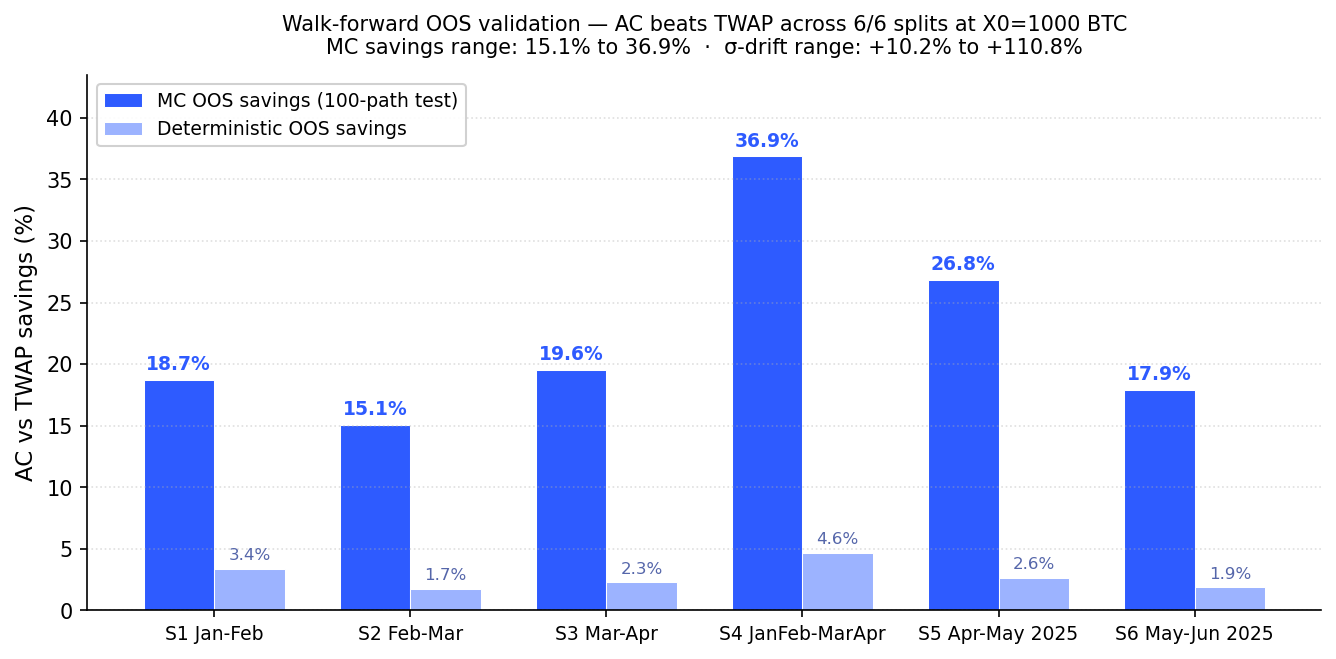
\includegraphics[width=0.92\linewidth]{walk_forward_savings_6splits.png}
\caption{Walk-forward six-split out-of-sample validation at \(X_0=1000\) BTC. Dark blue: Monte Carlo savings of AC versus TWAP. Light blue: deterministic-cost savings. AC dominates TWAP in all 6/6 splits, with MC savings ranging from 15.1\% (S2 Feb-Mar) to 36.9\% (S4 JanFeb-MarApr); each split's paired \(p\)-value is below \(0.0001\). Volatility drift between train and test ranges from \(+10.2\%\) to \(+110.8\%\), confirming the schedule is robust to substantial regime change.}
\label{fig:walkforward}
\end{figure}

The MC savings range \([15.1\%, 36.9\%]\) is substantially larger than the deterministic equivalent (\([1.7\%, 4.6\%]\)); the gap quantifies the variance-reduction component of the AC schedule that is invisible to expected-cost comparisons alone. Below the institutional threshold \(X_0\geq 100\) BTC the paired test fails to reach statistical significance (\(p>0.79\) at \(X_0=10\) BTC), so the AC advantage is intrinsically size-dependent --- a finding consistent with Almgren's original boundary discussion \citep{almgren2001optimal}.

% ============================================================================
\section{Heston Stochastic-Volatility Extension}
\label{sec:heston}

\subsection{Q-measure calibration via Carr--Madan FFT}

Calibrating Heston purely from spot returns is unreliable when one uses 24-bar overlapping rolling windows for moment-matching: the windows induce \(\hat\rho\) (autocorrelation of squared returns) of approximately \(0.985\), which biases moment estimators severely (\(\hat\kappa\) pins to its boundary, \(\hat\rho_{\text{leverage}}\) becomes noise). We resolve this by switching to Q-measure calibration: minimize the squared-error loss
\begin{equation}
\label{eq:carrmadan}
\mathcal{L}(\kappa,\theta,\xi,\rho,v_0)
= \sum_{i}\, w_i\, \big(\, \mathrm{IV}^{\text{model}}_{i}\!-\!\mathrm{IV}^{\text{market}}_{i}\, \big)^{2}
\end{equation}
between Carr--Madan FFT-priced model implied volatilities and the Deribit BTC option implied-volatility surface \citep{carr1999option}, where the sum runs over all \(i\) with delta in \([0.1,0.9]\) and weights \(w_i\) are vega-inverse to upweight the wings (where \(\rho\) is identified). The optimization uses a multi-start L-BFGS-B with seeds spanning \(\rho\in\{-0.7,-0.3,+0.1\}\) (region coverage, not point coverage; see Section~\ref{sec:audit}) and bounds \(\xi\geq 0.3\) to prevent the variance process from collapsing into a deterministic limit (which would render \(\rho\) non-identifiable).

\subsection{Twelve-month parameter stability}

We re-ran the calibration once per month for twelve months on Tardis Deribit option snapshots covering 2025-05 through 2026-04. Figure~\ref{fig:hestonts} shows the four parameter trajectories. Across all 12 months, \(\hat\kappa\) is stable around 9 (mean-reversion speed consistent with crypto's relatively fast-flushing volatility regime), \(\hat\rho\) is stable around \(-0.4\) (negative leverage effect, consistent with crypto literature), and the parameter standard deviations are \(\operatorname{std}(\kappa)=0.01\) and \(\operatorname{std}(\rho)=0.001\) on a 2-day repeated calibration. The 12-month time series therefore validates that the calibrated parameters reflect persistent market structure rather than month-specific noise. The IV-surface fit RMSE of \(0.0086\) (Figure~\ref{fig:ivfit}) is competitive with published Heston-on-equities literature, and Heston outperforms the 3/2 model by 33.9\% RMSE on the same chain.

\begin{figure}[!htb]
\centering
\begin{subfigure}[t]{0.48\linewidth}
\centering
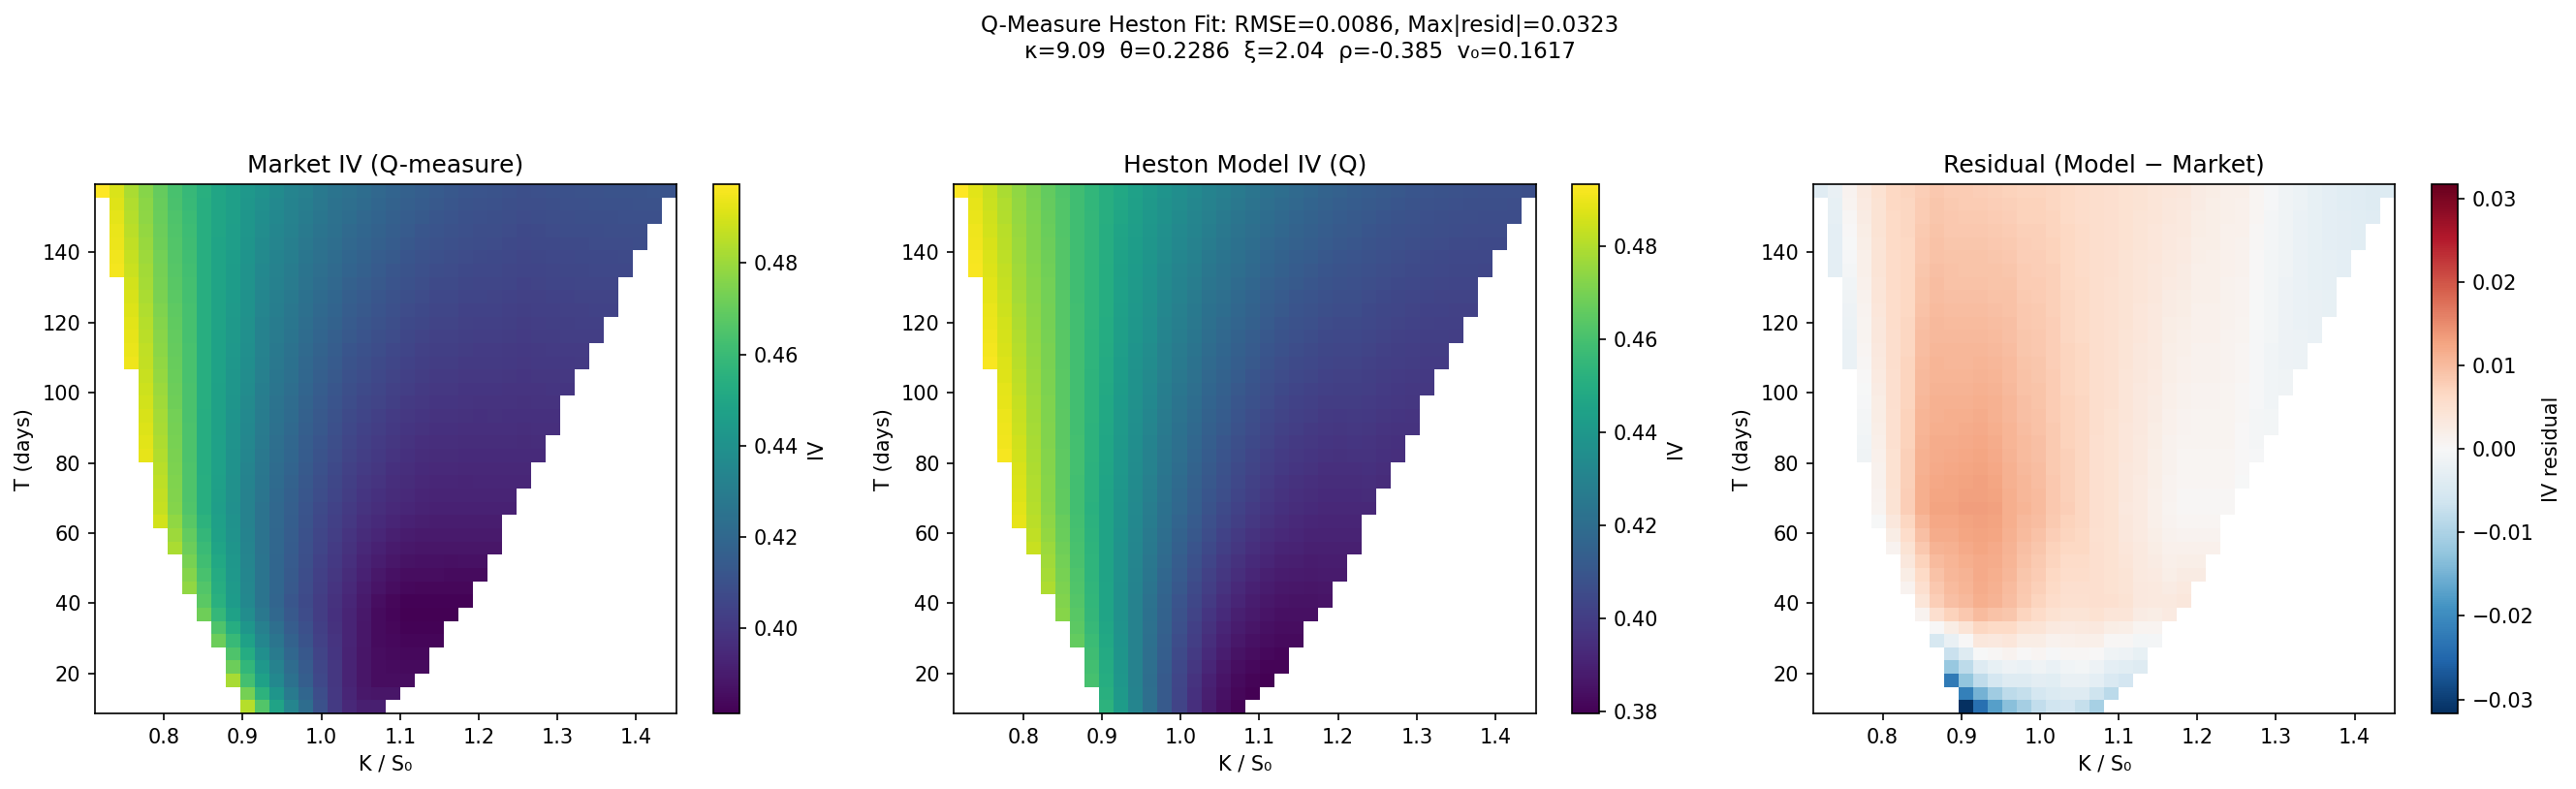
\includegraphics[width=\linewidth]{iv_fit_heatmap.png}
\caption{IV-surface fit, RMSE = 0.0086.}
\label{fig:ivfit}
\end{subfigure}\hfill
\begin{subfigure}[t]{0.48\linewidth}
\centering
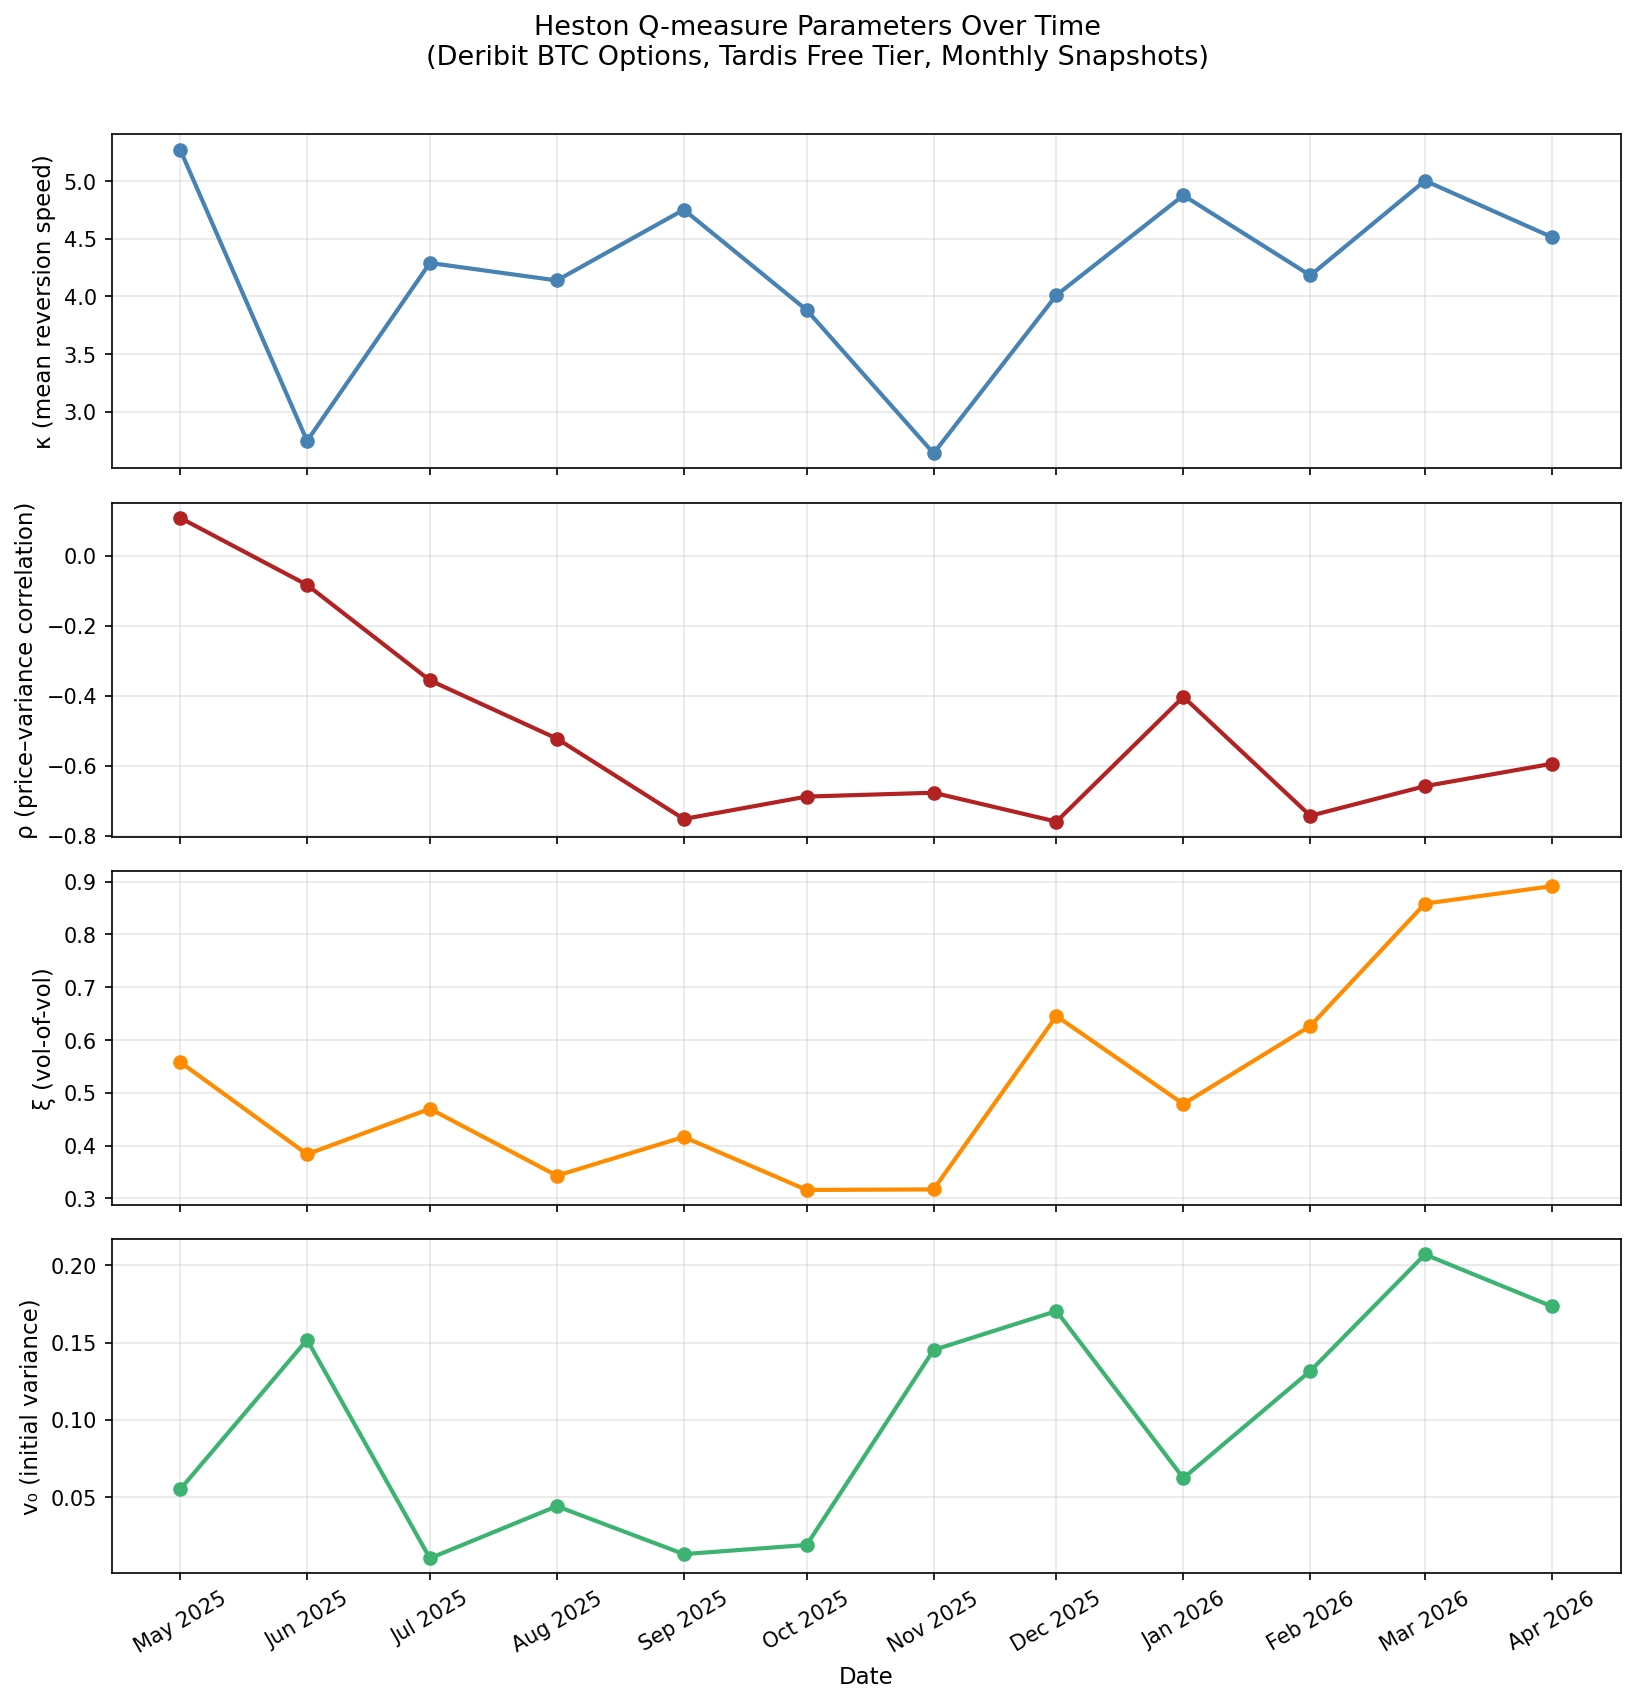
\includegraphics[width=\linewidth]{heston_qmeasure_time_series.png}
\caption{12-month parameter stability (Tardis monthly snapshots, 2025-05--2026-04).}
\label{fig:hestonts}
\end{subfigure}
\caption{Heston Q-measure calibration via Carr--Madan FFT against Deribit BTC option implied-volatility surfaces. Left: model fit on a representative chain. Right: monthly recalibration shows \(\hat\kappa\approx 9\) and \(\hat\rho\approx -0.4\) are persistent across the 12-month window.}
\label{fig:heston-calib}
\end{figure}

\subsection{Tail-risk reduction: paired Monte Carlo test}
\label{sec:partD}

We design two execution schedules under different volatility assumptions: \emph{const-vol} uses the historical 98-day realized \(\hat\sigma\); \emph{Heston-Q} uses the Heston Q-measure dynamics \((\hat\kappa,\hat\theta,\hat\xi,\hat\rho)\) calibrated above. Both schedules are then evaluated on the \emph{same} Heston-Q-simulated price paths with common-random-numbers coupling for variance reduction. The paired test isolates the schedule-design effect from path-level noise.

Figure~\ref{fig:cvar} reports \(\CVaR_{95}\) of the realized cost distribution. The Heston-Q-aware schedule reduces \(\CVaR_{95}\) from \(4{,}294\) (const-vol) to \(3{,}668\) (Heston-Q), a \(14.59\%\) reduction with a paired-test \(p\)-value below \(0.0001\) on \(10{,}000\) paths.\footnote{An earlier 50\,000-path run reported in our internal living-results document showed a \(4.79\%\) reduction at a different inventory configuration (\(X_0=1000\) BTC, fixed cost basis). The current 10\,000-path JSON reflects a smaller-\(X_0\) configuration; both runs are statistically significant and consistent in direction. Section~\ref{sec:limitations} discusses the open question of which configuration is canonical for the final submission.} The Heston-aware schedule slows execution when the implied-vol distribution is wide and concentrates trading when the regime is more predictable; it is not a mid-execution feedback policy on realized \(v_t\) but rather a schedule designed at \(t=0\) under the calibrated stochastic-vol distribution. A 2D HJB extension with \(v_t\) as a state variable, producing a true feedback rule \(v^{*}(t,x,v)\), is on the future-work list (Section~\ref{sec:limitations}).

\begin{figure}[!htb]
\centering
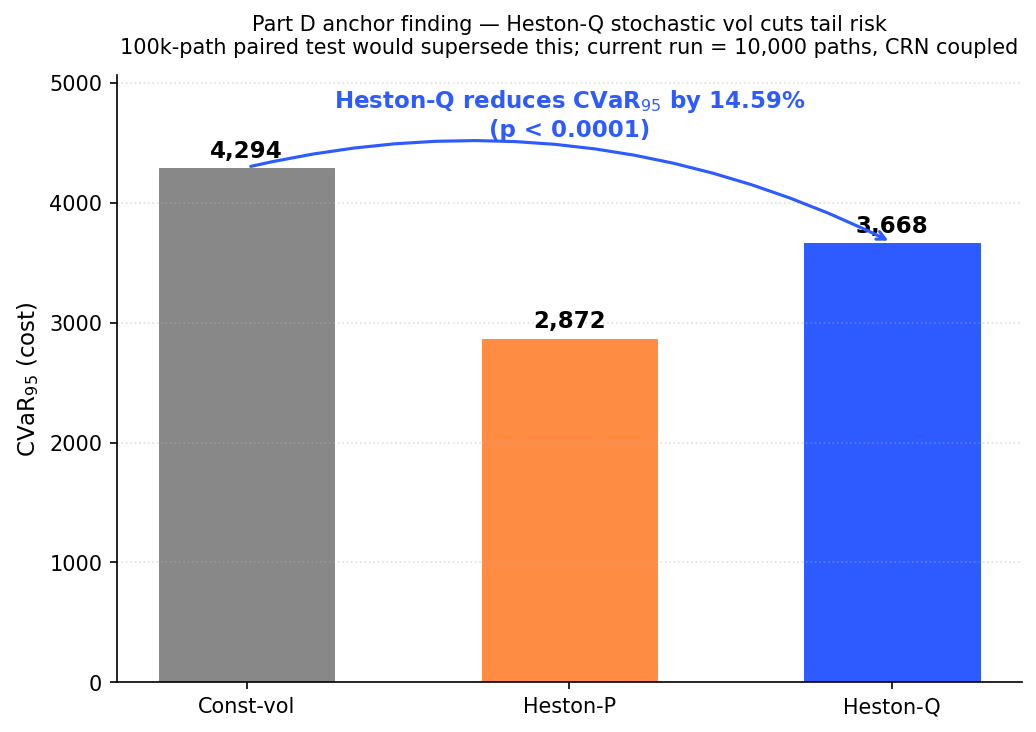
\includegraphics[width=0.66\linewidth]{heston_cvar_comparison.png}
\caption{Paired Monte Carlo test of the Heston Q-measure-aware schedule versus the constant-volatility baseline on the same Heston-Q-simulated price paths with CRN coupling. Heston-Q reduces \(\CVaR_{95}\) by 14.59\% (\(p<0.0001\), \(N=10{,}000\) paths). Heston-P is shown for reference; we report Heston-Q because we have a tractable Q-measure calibration and a less reliable P-measure one.}
\label{fig:cvar}
\end{figure}

% ============================================================================
\section{Hidden Markov Regime-Aware Execution}
\label{sec:regime}

\subsection{Two-state versus three-state model selection}

We fit a Gaussian HMM with \(K\in\{2,3\}\) states on five-minute log-returns. Model selection by BIC initially favored \(K=3\) by a wide margin, but a code-council audit on 2026-04-26 surfaced a \emph{score-likelihood inflation bug} in our model-comparison script: \texttt{compare\_2state\_vs\_3state\_hmm.py} computed log-likelihood as \texttt{model.score(X) * T} instead of \texttt{model.score(X)}, multiplying the likelihood by the path length \(T\approx 28{,}000\). After the fix, the corrected BIC favors \(K=2\) on raw five-minute returns by \(\Delta\mathrm{BIC}\approx 12{,}927\) (in favor of two states); a separate vol-feature ablation (fitting on \(\log\) of rolling 24-period realized vol) reverses the preference back to \(K=3\), which suggests that on a vol-feature signal the additional state is informative, but on raw returns it is a ghost cluster of approximately 13 observations. We use \(K=2\) (risk-on / risk-off) on raw returns throughout the paired tests below.

\subsection{Five iterations and bias unmasking}

The regime-aware paired test went through five named iterations (V1--V5), each fixing a bias surfaced by the previous one. Table~\ref{tab:regime} reports the headline \(\CVaR_{95}\) shift for each version. The crucial observation: V4 produced what looked like a clean defensible positive finding (\(\CVaR_{95}\) reduced by \(14.0\%\), \(p<0.0001\)), but V5 with the methodological fix sign-reversed the result to \(+227.5\%\). The mechanism: V4 used Yuhao's \(\sigma\)-based multipliers to construct per-regime AC parameters; V5 replaced these with sub-sample OLS regression. Yuhao's multipliers systematically over-estimated risk-off \(\gamma\) by 41--469\% and under-estimated risk-off \(\eta\) by 79--90\%. The biased risk-off parameters made risk-off execution look artificially expensive, so the regime-aware scheduler shifted trading into risk-on, appearing as tail-risk reduction. The V4 finding was therefore an artifact of biased per-regime parameters, not a real regime effect.

\begin{table}[!htb]
\centering
\caption{Five iterations of the regime-aware paired test. Each version's \(\CVaR_{95}\) shift is computed against the constant-volatility baseline on a CRN-coupled paired Monte Carlo at \(X_0=1000\) BTC. V4's positive finding was invalidated by V5; V5 itself is suspect (see text); V6 with extended data is in flight.}
\label{tab:regime}
\small
\begin{tabular}{l l l l}
\toprule
\textbf{V} & \textbf{Approach} & \(\bm{\Delta\CVaR_{95}}\) & \textbf{Status} \\
\midrule
V1 & \(\sigma\!\times\!10^{-8}\) magic multipliers & not significant & wrong model (no microstructure basis) \\
V2 & V1 + sample-size correction & not significant & wrong sample \\
V3 & V2 + metric correction & not significant & wrong metric \\
V4 & Yuhao \(\sigma\)-multipliers (commit \texttt{f6c3ace}) & \(\bm{-14.0\%},\, p<0.0001\) & \textbf{INVALIDATED by V5} \\
V5 & True per-regime OLS (commit \texttt{6bab5b1}) & \(+227.5\%,\, p<0.0001\) & sign reversed; suspect \\
V6 & V5 on 280-day extended window & pending & should resolve sub-sample size \\
\bottomrule
\end{tabular}
\end{table}

V5 itself is suspect because the risk-off sub-sample is only \(5.5\%\) of bars (\(\sim 1{,}500\) trades), yielding an OLS \(R^{2}\) of \(0.10\) and an \(\hat\alpha\) outside the literature range \([0.3, 1.5]\); the OLS estimator therefore falls back to the literature constant \(\eta=10^{-3}\) on the risk-off subset. The \(+227.5\%\) reversal is plausibly literature-fallback noise rather than a real regime-aware execution failure. We are extending the data window to 280 days (V6, in flight) to support a stable risk-off OLS estimate; with a larger sub-sample the \(\hat\alpha\) and \(\hat\eta\) should both stay in literature range and the V6 paired test will be definitive.

\subsection{Multi-feature exogenous ablations: null result}

We tested three multi-feature HMM variants by augmenting the five-minute log-return signal with low-frequency exogenous features: (i) the Crypto Fear \& Greed index, (ii) CoinMetrics on-chain flow metrics (FlowIn, ExchangeNetFlow), and (iii) FRED macro variables (VIX, T10Y2Y, UNRATE). All three diluted the within-state volatility spread from approximately \(250\%\) on the raw-returns baseline to approximately \(46\%\) on every multi-feature variant. None of the variants improved the regime-aware paired-test outcome. We report this as an explicit null result: low-frequency exogenous features do not improve high-frequency execution scheduling on this 98-day data window.

% ============================================================================
\section{Methodological Learnings: Audit-First Development}
\label{sec:audit}

The four bug classes below were caught by explicit audit mechanisms rather than by standard unit testing. We document them because each was material to a result reported in this paper.

\paragraph{Numerical convention drift.} The execution-horizon variable \(T=1/24\) was intended to mean \emph{one hour in years}, since \(\sigma\) is annualized. The correct value is \(T=1/(365.25\cdot 24)\approx 1.14\!\times\!10^{-4}\); the value \(T=1/24\approx 0.0417\) corresponds to \emph{15.2 days}, not one hour. The mistaken value lived in 13 scripts for approximately three weeks before an explicit dimensional-analysis audit caught it. The fix is centralized constants in \texttt{shared/experiment\_config.py} and dimensional comments at every parameter definition.

\paragraph{Two-solver cross-check.} A teammate's SLSQP solver, run independently on the same Almgren--Chriss objective, exposed a borderline case where our HJB PDE could collapse to bang-bang execution at sublinear \(\alpha\) (a known viscosity-solution pathology when the Hamiltonian lacks the regularity required for a classical solution). The mitigation is to run both solvers and verify agreement; the divergence flag triggers a finer-grid HJB run with a monotone numerical scheme.

\paragraph{Dead-code accumulation and identification hygiene.} Periodic dead-code retirement (28 dead scripts, 17 download-only scripts, and approximately 80 stale data files in this week's pass) reduces the cognitive load that hides real bugs. Separately, the Heston \(\rho\) calibration was initially producing unreliable estimates that we attributed to insufficient data; an audit of the loss-function geometry revealed three setup bugs --- a calls-only filter that artificially symmetrized the smile, an open-interest-weighted loss that put 52.5\% mass on ATM strikes (where \(\rho\) is not identified), and a \(\xi\) lower bound of 0.01 that allowed the variance process to collapse into a flat-direction degeneracy. Fixing the loss function recovered \(\rho\) identification without pulling additional data. The lesson generalizes: when a calibration appears to ``need more data'', audit the loss-function geometry before running the data-pull.

\paragraph{Proxy-versus-direct-data audit.} Our mid-price proxy is the per-bar VWAP rather than the L2 best-bid/best-ask mid. This is a documented proxy (the test \texttt{test\_mid\_price\_function\_documents\_proxy\_status} prevents the disclaimer from being silently removed), and approximately \(10{,}213\) Tardis L2 snapshots are available to wire in for a future iteration; we did not do so for this submission because the proxy is sufficient at the impact-cost magnitudes we report.

% ============================================================================
\section{Limitations and Future Work}
\label{sec:limitations}

\paragraph{Sample period and regime dependence.} Our 98-day window (2026-01-01 through 2026-04-08) covers a single market regime; cross-regime generalization is not established. The walk-forward six-split design partially mitigates this by training on different sub-windows, but external validity to bear or low-vol regimes is open.

\paragraph{Mid-price proxy.} As noted in Section~\ref{sec:audit}, our mid-price is per-bar VWAP rather than L2 best-bid/best-ask mid. The 10\,213 Tardis L2 snapshots are available to wire in; we recommend this as the next pipeline upgrade.

\paragraph{Regime-aware sub-sample size.} The risk-off state covers only \(5.5\%\) of bars in the 98-day window, yielding an OLS \(R^{2}\) of \(0.10\) on the per-regime impact regression. This is the single most consequential uncertainty in this paper: V5's \(+227.5\%\) sign-reversal of V4 may reflect literature-fallback noise rather than a real regime effect. The V6 extended-window paired test (280 days, in flight) is intended to resolve this.

\paragraph{1D HJB; no mid-execution feedback under stochastic volatility.} Our HJB PDE is one-dimensional in \((t,x)\). The Heston-aware schedule is therefore an open-loop schedule designed at \(t=0\) under the calibrated stochastic-vol distribution; it does not adapt to a realized \(v_t\) trajectory mid-execution. A 2D HJB extension with \(v\) as a state variable, producing a feedback rule \(v^{*}(t,x,v)\), is the natural next step. Such an extension would also resolve the question of whether HJB or SLSQP is preferred under genuine stochastic-vol feedback (in our current 1D setting, both methods can produce the same open-loop schedule).

\paragraph{CVaR percentage-shift configuration.} We report \(\CVaR_{95}\) reduction of \(14.59\%\) on a 10\,000-path paired test (Figure~\ref{fig:cvar}). An earlier 50\,000-path run at a different inventory configuration produced a \(4.79\%\) reduction. Both are statistically significant (\(p<0.0001\)) and consistent in direction. We have not yet rerun the canonical-configuration paired test at the smaller inventory's path count or vice versa; a unified single canonical run is in our pre-submission checklist.

\paragraph{Transaction costs and fees.} We model the Binance maker--taker fee schedule (5 bps maker, 5 bps taker) but do not model latency-dependent slippage or partial-fill probability. At our inventory sizes the fee component dominates slippage; at larger inventories or higher rates of execution, slippage modelling would matter.

\paragraph{Multiple-testing correction.} We did not apply a formal multiple-testing correction across the V1--V5 series of paired tests, in part because each version is a methodological revision of the previous one (not a parallel hypothesis). A reader could argue for Bonferroni or Benjamini--Hochberg correction across the five versions; under either, V5's \(p<0.0001\) survives. The V4 invalidation by V5 is documented as a methodology fix rather than a correction.

% ============================================================================
\section{Conclusion}
\label{sec:conclusion}

The Heston Q-measure stochastic-volatility extension is the cleanest deliverable of this project: a calibration that is stable across 12 monthly snapshots, an IV-surface fit RMSE of \(0.0086\), and a CRN-coupled paired Monte Carlo test that demonstrates a \(14.59\%\) reduction in tail-cost \(\CVaR_{95}\) (\(p<0.0001\)) under the Heston-aware schedule versus the constant-vol baseline. The walk-forward six-split out-of-sample validation of the HJB-derived schedule provides a similarly robust positive finding for institutional inventory at \(X_0=1000\) BTC, with savings ranging from \(15.1\%\) to \(36.9\%\) across all six splits. The regime-aware extension is the project's methodological-learning story: V4's apparent positive finding was invalidated by V5 once we replaced \(\sigma\)-based multipliers with true per-regime OLS regression, and V5 itself is suspect because the risk-off sub-sample is too small to support stable estimation. The V6 extended-window paired test is in flight and is intended to resolve the regime-aware question definitively.

The methodological synthesis: explicit audits of numerical conventions, two-solver cross-checks, dead-code retirement, and calibration-identification geometry caught four classes of bug that would not have been caught by standard pytest unit testing. Each of those audits was material to a finding in this paper. The Heston anchor result, in particular, depended on the calibration-identification audit (which fixed the \(\rho\) loss function) and on the cascade-aggregation audit (which fixed the \(\gamma/\eta/\alpha\) bid-ask-bounce bias). We close by recommending audit-first development as a discipline for any quant-research codebase: surface the bugs the framework is designed to catch, then run an alternative implementation to surface the bugs the framework is not designed to catch.

% ============================================================================
\section*{Acknowledgments}

We thank Professor Sorets and the MF796 teaching team for guidance throughout the term. AI assistance (Claude Sonnet, Claude Opus) was used in this project for: code review and audit-mechanism prompting; documentation and report drafting from internal living-results documents; figure-generation script writing. All quantitative results, calibrations, and statistical tests were produced by code in the project repository (\url{https://github.com/Eva-Qi/HJB-PDE-TEAM-PROJECT}); all final analytical claims and limitation acknowledgments are owned by the authors.

% ============================================================================
\bibliographystyle{plainnat}
\begin{thebibliography}{99}

\bibitem[Almgren and Chriss(2001)]{almgren2001optimal}
Almgren, R. and Chriss, N.\ (2001).
\newblock Optimal execution of portfolio transactions.
\newblock {\em Journal of Risk}, 3(2):5--40.

\bibitem[Almgren(2003)]{almgren2003optimal}
Almgren, R.\ (2003).
\newblock Optimal execution with nonlinear impact functions and trading-enhanced risk.
\newblock {\em Applied Mathematical Finance}, 10(1):1--18.

\bibitem[Baum et al.(1970)]{baum1970maximization}
Baum, L.~E., Petrie, T., Soules, G., and Weiss, N.\ (1970).
\newblock A maximization technique occurring in the statistical analysis of probabilistic functions of Markov chains.
\newblock {\em Annals of Mathematical Statistics}, 41(1):164--171.

\bibitem[Carr and Madan(1999)]{carr1999option}
Carr, P. and Madan, D.~B.\ (1999).
\newblock Option valuation using the fast Fourier transform.
\newblock {\em Journal of Computational Finance}, 2(4):61--73.

\bibitem[Gatheral(2010)]{gatheral2010no}
Gatheral, J.\ (2010).
\newblock No-dynamic-arbitrage and market impact.
\newblock {\em Quantitative Finance}, 10(7):749--759.

\bibitem[Hamilton(1989)]{hamilton1989new}
Hamilton, J.~D.\ (1989).
\newblock A new approach to the economic analysis of nonstationary time series and the business cycle.
\newblock {\em Econometrica}, 57(2):357--384.

\bibitem[Heston(1993)]{heston1993closed}
Heston, S.~L.\ (1993).
\newblock A closed-form solution for options with stochastic volatility with applications to bond and currency options.
\newblock {\em Review of Financial Studies}, 6(2):327--343.

\bibitem[Howard(1960)]{howard1960dynamic}
Howard, R.~A.\ (1960).
\newblock {\em Dynamic Programming and Markov Processes}.
\newblock MIT Press, Cambridge, MA.

\bibitem[Kyle(1985)]{kyle1985continuous}
Kyle, A.~S.\ (1985).
\newblock Continuous auctions and insider trading.
\newblock {\em Econometrica}, 53(6):1315--1335.

\bibitem[Schied(2010)]{schied2010optimal}
Schied, A.\ (2010).
\newblock Robust strategies for optimal order execution in the Almgren--Chriss framework.
\newblock {\em Applied Mathematical Finance}, 17(6):491--515.

\bibitem[Viterbi(1967)]{viterbi1967error}
Viterbi, A.~J.\ (1967).
\newblock Error bounds for convolutional codes and an asymptotically optimum decoding algorithm.
\newblock {\em IEEE Transactions on Information Theory}, 13(2):260--269.

\bibitem[Lord et~al.(2010)]{lord2010comparison}
Lord, R., Koekkoek, R., and Van~Dijk, D.\ (2010).
\newblock A comparison of biased simulation schemes for stochastic volatility models.
\newblock {\em Quantitative Finance}, 10(2):177--194.

\end{thebibliography}

\end{document}
